\documentclass{article}
\usepackage[left=2cm, right=2cm, top=2cm]{geometry}
%%%%%%%%%%%%%%%%%%%%%%%%%%%%%%%%%% PACKAGES %%%%%%%%%%%%%%%%%%%%%%%%%%%%%%%%%%
\usepackage{minted}                     % Code
\usepackage{graphicx}                   % PNGs
\usepackage{algorithm}
\usepackage{algpseudocode}              % Algorithms
\usepackage{amsmath}                    % Rightarrow
\usepackage{hyperref}                   % Hyperlinks
\hypersetup{
    colorlinks,
    linkcolor=black
}

%%%%%%%%%%%%%%%%%%%%%%%%%%%%%%%%%%%%%%%%%%%%%%%%%%%%%%%%%%%%%%%%%%%%%%%%%%%%%%%

\pagenumbering{gobble}

\title{\textbf{Final Project}}
\author{MacMillan, Kyle}
\date{December 11, 2018}


\begin{document}

\maketitle
\addcontentsline{toc}{section}{Title}

\newpage
\pagenumbering{roman}   % Set TOC page numbering to lowercase roman numerals
\tableofcontents
\addcontentsline{toc}{section}{Table of Contents}

\newpage
\listoffigures
\addcontentsline{toc}{section}{List of Figures}

\newpage
\pagenumbering{arabic}  % Set content page numbering to arabic numerals
% Setup Hyperlinks for the rest of the document
\hypersetup{
    colorlinks,
    citecolor=blue,
    filecolor=black,
    linkcolor=blue,
    urlcolor=blue
}

\section{Description of the program}
\setcounter{page}{1} % Set the page counter to 3
This write-up is for the 
\href{https://www.mcs.sdsmt.edu/ckarlsso/csc410/fall18/csc410_Final.pdf}{Final project} 
and the repository for my work is 
\href{https://github.com/macattackftw/HighPerfComputing/tree/master/final}{here} 
and 
\href{https://github.com/macattackftw/HighPerfComputing/tree/master/seqfinal}{here}.
\\

This program was incredibly hard until I learned of \verb|std::next_permutation|
. Until then I had a ridiculous chain of nested for loops to iterate over up to 
$n = 10$. Also, because it was a nested loop I had to do a horizontal check to 
ensure there were not duplicate queens on a line. This made the program 
unbearably slow. Joe informed me of \verb|std::next_permutation| and it was a 
complete game changer. 

Armed with this new tool I began to design a solution capable of using it. After 
searching around online I found a 
\href{https://stackoverflow.com/a/7919887}{Stack Overflow post} that allowed me 
to calculate the $i^{th}$ permutation. Given $p$ processors and a known number 
of permutations given in the form of $n!$ I can calculate the number of 
permutations to send to each processor. This is not the \textit{best} load 
balance strategy, but it is not terrible. Since I am not pruning the 
permutations the only imbalance comes from transmitting that a valid board 
layout was found.

The graduate portion of this assignment allowed me to utilize a Task/Channel 
method (as described in Chapter 6) to complete the assignment. By having 
\verb|MPI_Send| and \verb|MPI_Recv| in the workers and master, respectively, I 
was able to meet that program requirement. Essentially the master goes directly 
into a receive loop, waiting for an \verb|MPI_Send| on the appropriate tag and 
source. After receiving the value a counter is incremented and it checks if we 
have hit the expected number of solutions. If we have not finished it goes back 
into the receive loop, otherwise it sends out an \verb|MPI_Bcast| to all workers 
that changes a boolean flag from $false$ to $true$, which stops them from 
checking any more boards.

\subsection{Performance Analysis}
Timing was performed with the simple Linux \verb|time| command. This problem is 
not like our previous assignments. We have an exponential growth in the problem 
size \textit{at each step}. That means we don't really need high-fidelity timing 
to get a picture of what's going on. 

Figure \ref{fig:seq11} shows that up to $n=11$ my sequential implementation is 
faster than the MPI solution shown in Figure \ref{fig:mpi11}. I didn't give it 
much thought at first and decided to try and run the problem on a ``single'' 
processor but I had left the host file filled with computers so I am not sure 
what the numbers in Figure \ref{fig:mpiseq11} represent. After that blooper I 
created the sequential code which is a clone of the \verb|MPI| with all 
\verb|MPI| aspects stripped out. 

\begin{figure}[h]
    \centering
    \begin{minipage}{0.49\textwidth}
        \centering
        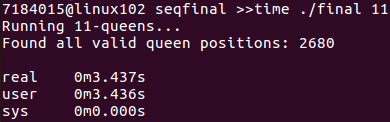
\includegraphics[width=0.75\textwidth]{MPI_2_11}
        \caption{Sequential 11-queens}
        \label{fig:seq11}
    \end{minipage}\hfill
    \begin{minipage}{0.49\textwidth}
        \centering
        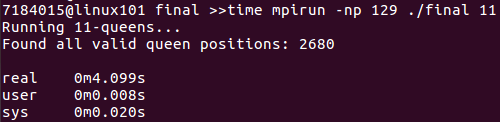
\includegraphics[width=0.95\textwidth]{MPI_11}
        \caption{MPI 11-queens}
        \label{fig:mpi11}
    \end{minipage}
\end{figure}


\begin{figure}[h]
    \centering
    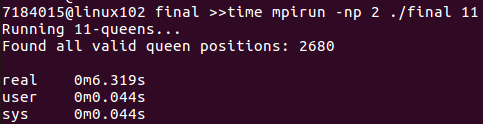
\includegraphics[width=0.5\textwidth]{MPI_1_11}
    \caption{``Sequential'' MPI 11-queens}
    \label{fig:mpiseq11}
\end{figure}

\begin{figure}[h]
    \centering
    \begin{minipage}{0.49\textwidth}
        \centering
        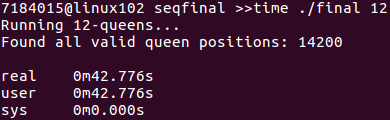
\includegraphics[width=0.75\textwidth]{MPI_2_12}
        \caption{Sequential 12-queens}
        \label{fig:seq12}
    \end{minipage}\hfill
    \begin{minipage}{0.49\textwidth}
        \centering
        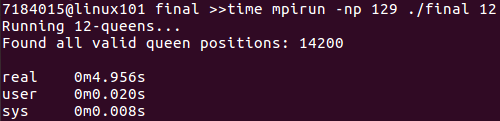
\includegraphics[width=0.95\textwidth]{MPI_12}
        \caption{MPI 12-queens}
        \label{fig:mpi12}
    \end{minipage}
\end{figure}

Figure \ref{fig:seq12} shows the sequential time for $n=12$ and Figure 
\ref{fig:mpi12} shows the first time the MPI solution beat the sequential 
solution, and it was by quite a margin.

\begin{figure}[h]
    \centering
    \begin{minipage}{0.49\textwidth}
        \centering
        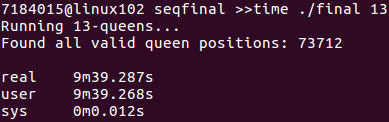
\includegraphics[width=0.75\textwidth]{MPI_2_13}
        \caption{Sequential 13-queens}
        \label{fig:seq13}
    \end{minipage}\hfill
    \begin{minipage}{0.49\textwidth}
        \centering
        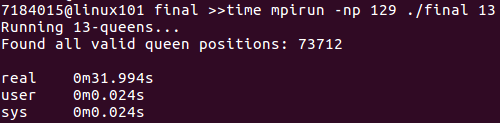
\includegraphics[width=0.95\textwidth]{MPI_13}
        \caption{MPI 13-queens}
        \label{fig:mpi13}
    \end{minipage}
\end{figure}

Wanting to gather as much data as possible I ran sequential up to $n=13$. Figure 
\ref{fig:seq13} shows that it took 9 minutes and 39 seconds to quit early from a 
sequential run of $n=13$. Figure \ref{fig:mpi13} shows it took 18 times longer 
to run the sequential compared to \verb|MPI|. I calculated out the estimated 
sequential time for $n=14$ at 135.1 minutes for sequential code.

\begin{figure}[h]
    \centering
    \begin{minipage}{0.49\textwidth}
        \centering
        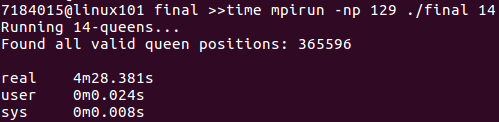
\includegraphics[width=0.95\textwidth]{MPI_14}
        \caption{MPI 14-queens}
        \label{fig:mpi14}
    \end{minipage}\hfill
    \begin{minipage}{0.49\textwidth}
        \centering
        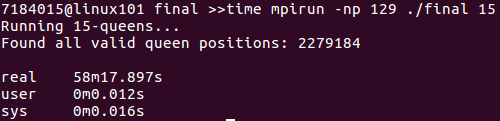
\includegraphics[width=0.95\textwidth]{MPI_15}
        \caption{MPI 15-queens}
        \label{fig:mpi15}
    \end{minipage}
\end{figure}

\section{Description of the algorithms and libraries used}
The STL's \verb|next_permutation| was a keystone in the design and execution of 
this program. \verb|MPI| was used. The 
\href{https://stackoverflow.com/a/7919887}{Stack Overflow post} for $n^{th}$ 
permutation was incredibly useful.

\section{Description of functions and program structure}
\subsection{Program Structure}
This program was setup with a Master/Slave (aka worker) configuration. The 
Master in this case was \verb|linux102| or \verb|linux103| and the workers were 
\verb|linux01-16|. I love classes so I wrote this in \verb|C++| and included a 
\href{}{Board} class. Essentially when the program fires up it verifies user 
input and then spins up the Master/Worker relations. Master eagerly awaits 
\verb|MPI_Send| commands from the workers and then updates the ``found'' count. 
Once the count reaches the threshold for this $n$-queens problem the Master uses 
\verb|MPI_Bcast| to change a boolean flag which causes the workers to shutdown. 

There is a ``feature'' I left in the code that causes crashes. I tried 
everything I could think of but due to the graduate requirement of early exit it 
completely messes with the \verb|MPI_Send| and \verb|MPI_Recv|. I tried all 
kinds of combinations to get it to exit cleanly but if you put too many 
processors on a small problem it will hang for a minute then dump. My 
\verb|MPI_Send| was only being called on success. That leaves the Master hanging 
in a receive loop.

Sequential works a little different in that instead of a Master/Worker 
relationship it has these 8 lines of code:

\begin{minted}{c++}
    uint8_t *queens = (uint8_t*)malloc(n * sizeof(uint8_t));
    for (uint8_t i = 0; i < n; ++i){
        queens[i] = i;
    }
    std::cout << "Running " << int(n) << "-queens..." << std::endl;
    SBoard b(factorials[n], n, print_out, queens);
    b.validSBoardPermutations();
    free(queens);
\end{minted}

There are two helper \verb|.h| files: \verb|completion.h| and 
\verb|nthpermutation.h|. The helper files contain constants and functions 
relevant to completion of tasks as well as the code to calculate the $n^{th}$ 
permutation.

\subsection{Description of Functions}
Each function has a header if you wish to know details. Please see my repository 
\href{https://github.com/macattackftw/HighPerfComputing/tree/master/final}{here} 
and 
\href{https://github.com/macattackftw/HighPerfComputing/tree/master/seqfinal}{here} 
for \verb|MPI| and sequential solutions respectively.

\newpage
\section{How to compile and use the program}
\subsection{MPI Run}
This program can be compiled with the Makefile. From the `final' folder simply 
type: 
$$\texttt{make}$$
$$or$$
$$\texttt{make final}$$

\noindent To use the program type:
$$\verb|mpirun -np 129 .\final 13|$$
$$or$$
$$\verb|mpirun -np 129 .\final 13 printout|$$

`129' represents the number of processors and `13' represents the $n$ part of 
the n-queens problem. Master node $id = 0$, therefore it is necessary to run 
with \verb|-np 2| or more. It \textbf{will not run properly} if you specify 
\verb|-np 1|. If you wish to run it sequentially see Section 
\ref{sec:sequential}. The \verb|printout| must follow the integer and is used to 
print valid queen positions to the console if you wish to have printouts.


\subsection{Sequential}\label{sec:sequential}
This program can be compiled with the Makefile. From the `seqfinal' folder 
simply type: 
$$\texttt{make}$$
$$or$$
$$\texttt{make final}$$

\noindent To use the program type:
$$\verb|.\final 10|$$
$$or$$
$$\verb|.\final 10 printout|$$

\verb|10| can be any integer, though I do not recommend going above 12 because 
run time is likely to exceed 9 minutes as shown in Figure \ref{fig:seq13}. The 
\verb|printout| must follow the integer and is used to print valid queen 
positions to the console if you wish to have printouts.

\newpage
\section{Description of the testing and verification process}{\label{sec:test}}
Testing was done with printout verification and count verification. I send the 
valid queen positions to console and verified them by hand. Figure 
\ref{fig:console} shows an example printout. This could obviously only be done 
on smaller $n$ values. For larger $n$ values I assumed the diagonal check was 
correct and only verified with the count method. A 
\href{https://github.com/macattackftw/HighPerfComputing/blob/master/final/include/completion.h#L15}{correctCount} 
function was made to test the count against a 
\href{https://github.com/macattackftw/HighPerfComputing/blob/master/final/include/completion.h#L7}{const array} 
of known solutions for a given $n$.

\begin{figure}[h]
    \centering
    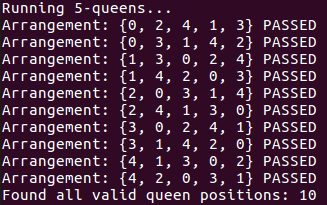
\includegraphics[width=0.5\textwidth]{console_output}
    \caption{Testing n-queens output}
    \label{fig:console}
\end{figure}

\section{Description of what you have submitted}
Included in the submission is the code needed to compile the program, two 
Makefiles to compile said code, and a detailed write-up of the assignment in pdf 
form.

\section{Additional Thoughts}
I really wish we had more time for this project. I would have really liked to 
dig into \verb|MPI| more; it's extremely powerful. I wanted to go about this 
problem in a totally different route but I was time constrained (due to 
coursework and personal reasons). 

Ideally I believe this problem would be solved with an \verb|MPI_Send| and 
\verb|MPI_Recv| in each worker. Instead of splitting the entire set of 
permutations amongst $p$ processors I wanted to split \textit{half} of the 
permutations amongst $p$ processors. Then when one finished early through 
\textit{pruning} it could push an \verb|MPI_Send| call to the Master node, at 
which point it would \verb|MPI_Recv| the request and \verb|MPI_Send| a new 
permutation along with $k$ permutations to run through. What this would have 
accomplished was essentially a worker queue so as workers finished they would 
request more work. Given that this problem has very dynamic work loads this 
would be a ``near-ideal'' plan.

I wanted to do pruning but it added more complexity than I was willing to commit 
to with the time available. It'd be really neat to have a 
``Distributed Computing'' or ``Parallel 2'' course that built on \verb|CUDA| and 
\verb|MPI|.

Overall fun course and I may be able to use \verb|MPI| for my thesis work.

\end{document}
